\paragraph{Vertical Displacement $\delta$}

When an obstacle hexagon is rotated by $\alpha_i$, the height of the hexagon becomes $2 N(n,m) \sqrt{3} \sec \alpha_i$.

\begin{minipage}{\linewidth}
\begin{center}
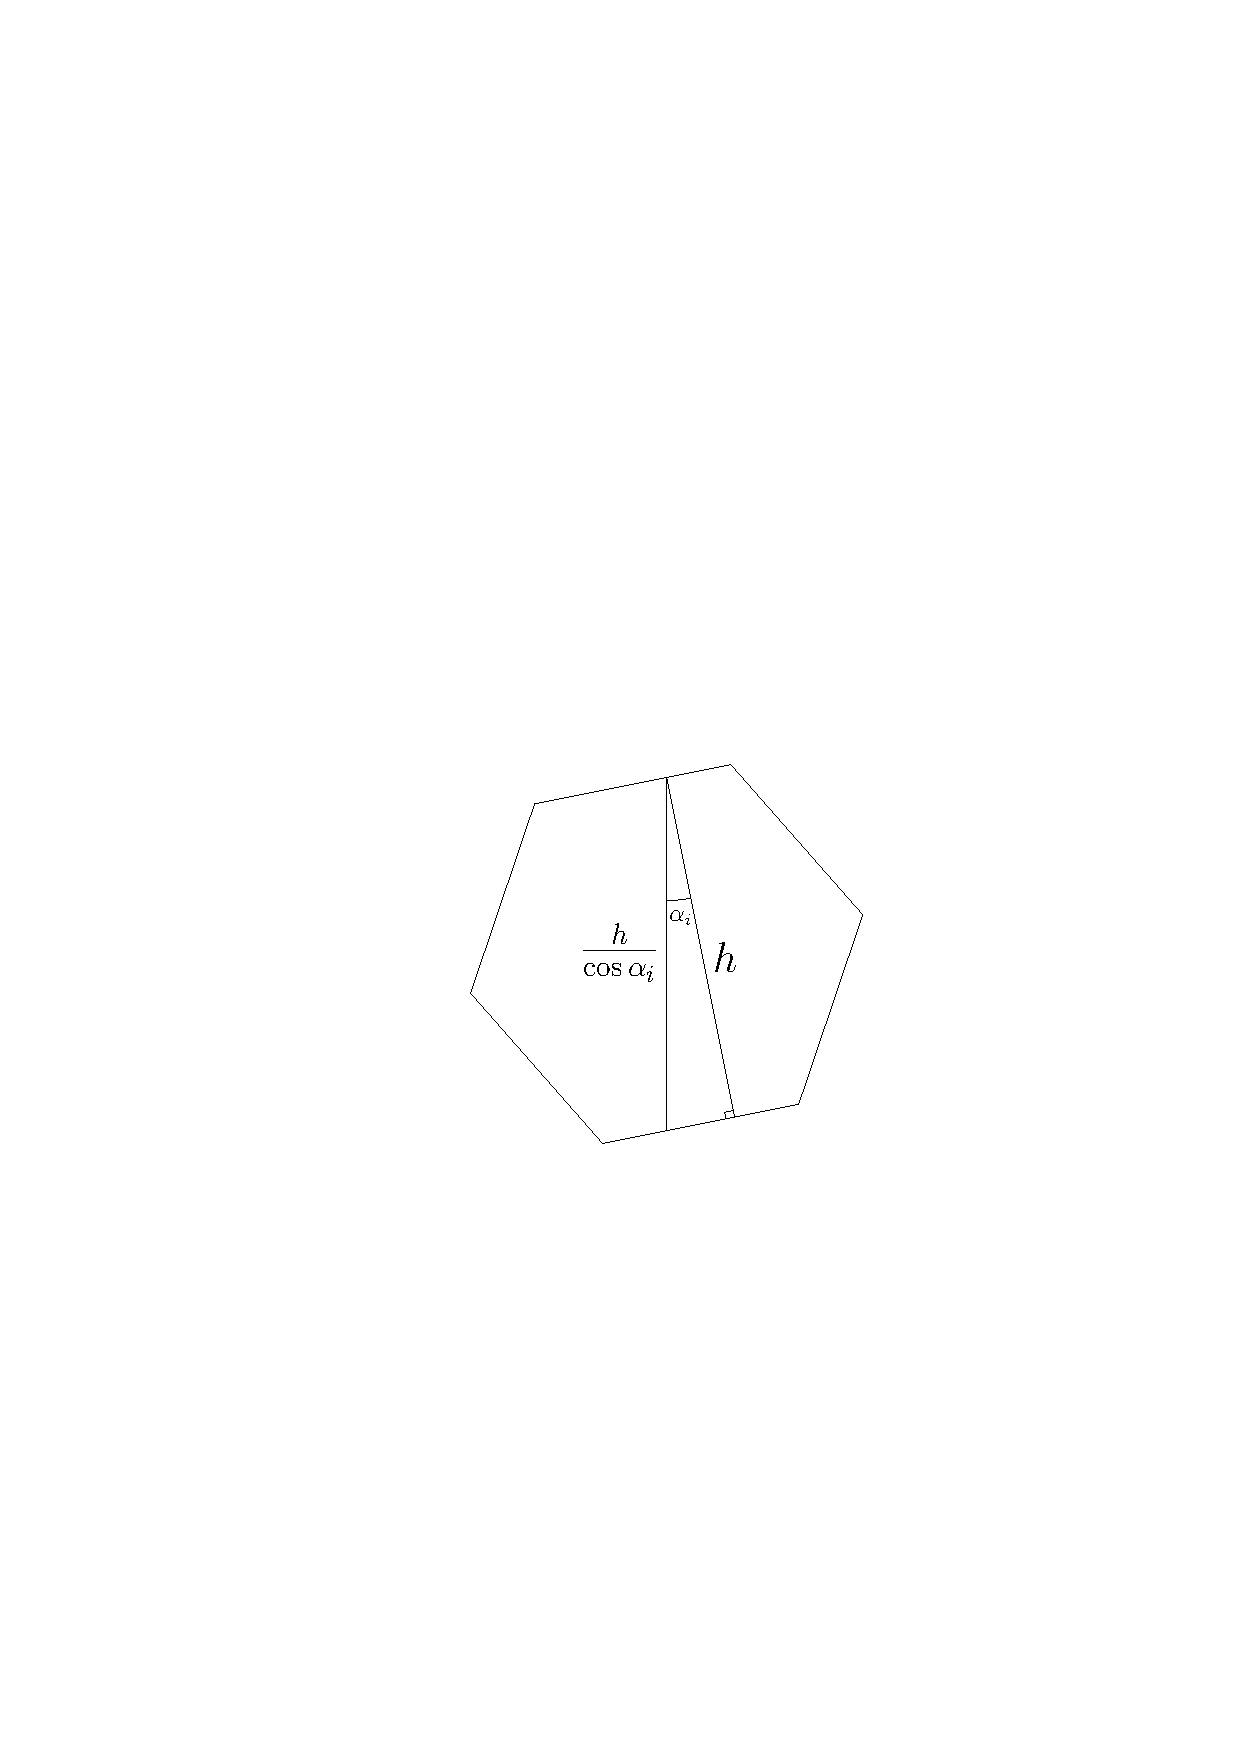
\includegraphics[width=.33\columnwidth]{graphics/hexagonNonCanonical2.pdf}
\captionof{figure}{
% The obstacle hexagon here is in non-canonical position, and showing the side lengths adjacent to $\alpha_i$.
This figure shows a right triangle with angle $\alpha_i$ and sides of length $h$ and $\frac{h}{\cos \alpha_i}$.
}\label{fig:hexagonNonCanonical.pdf}
\end{center}
\end{minipage}

%The height of the cross section of an obstacle polygon and  
Figure \ref{fig:hexagonNonCanonical.pdf} shows the geometry of a rotated obstacle hexagon.%height of the obstacle hexagon is $2 N(n,m) \sqrt{3}$.  
Using Equation \ref{eqn:Hnm} of $H(n,m)$, the length from the canonical position can also be represented as a sum of widths of corridors and cross sectional heights obstacle hexagons in arbtrary position.
We use this to bound the height of an arbitrary modified auxilary construction:
\begin{eqnarray*}
3 z \lr{\frac{1}{100N} + \sqrt{3}} + 2 N \sqrt{3} \sum_{i=1}^{3z+1} \sec \alpha_i &\leq& 3z \lr{\frac{1}{100N} + \sqrt{3}} + (3z+1) 2 N \sqrt{3}\\
 2 N \sqrt{3} \sum_{i=1}^{3z+1} \sec \alpha_i &\leq& (3z+1) 2 N \sqrt{3}\\
\sum_{i=1}^{3z+1} \sec \alpha_i &\leq& (3z+1)\\
&\leq& \sum_{i=1}^{3z+1} \lr{1 + \frac{a_i^2}{2}}\\
&=& 3z+1 + \sum_{i=1}^{3z+1}  \frac{a_i^2}{2}
\end{eqnarray*}
Note that $\left\vert \sec \alpha_i \right\vert \geq 1$.

%%%%%%%%%% COPA VIDA COMMENT OUT ON SATURDAY %%%%%%%%%%
% \begin{eqnarray*}
% H(n,m) = (u+1) \frac{5t-1}{2} \sqrt{3} + u \lr{\frac{1}{100N} + \sqrt{3}}&=& \sum_{i=1}^{u} \sqrt{3} + \sum_{i=1}^{u+1} \frac{5t-1}{2}\sqrt{3} \sec \alpha_i \\ 
% &\leq& u \sqrt{3} + \frac{5t-1}{2} \sqrt{3} \sum_{i = 1}^{u+1} \sec \alpha_i\\
% u \lr{\frac{1}{100N} + \sqrt{3} - \sqrt{3} } &\leq&(t+1) \sqrt{3}    \sum_{i = 1}^{u+1}  \lr{\sec \alpha_i - 1}\\
% \frac{u}{100N(t+1)\sqrt{3}}&\leq& \sum_{i = 1}^{u+1} \lr{1 + \frac{\alpha_i^2}{2} - 1}\\
% \frac{2u}{100N(t+1)\sqrt{3}}&\leq& \sum_{i = 1}^{u+1} \alpha_i^2\\
% \sqrt{\frac{2u}{100N(t+1)\sqrt{3}}} &\leq& \sum_{i=1}^{u+1} \alpha_i\\
% \sqrt{\frac{2u}{100N(t+1)\sqrt{3}}} &\leq& \sum_{i=1}^{u+1} \alpha_i + \alpha_i - \alpha_i\\
% \sum_{i=1}^{u+1} \alpha_i + \alpha_i - \alpha_i &\leq& \sum_{i=1}^{u+1} \alpha_i + \frac{3N^2 - 4 - \frac{4}{(100N)^2}}{N^3}
% \end{eqnarray*}
% Which implies:
% $$\sqrt{\frac{2u}{100N(t+1)\sqrt{3}}} \leq \sum_{i=1}^{u+1} \alpha_i  \leq (u+1) \lr{\frac{3N^2 - 4 - \frac{4}{(100N)^2}}{N^3}}$$
% \begin{eqnarray*}
%%%%%%%%%% COPA VIDA COMMENT OUT ON SATURDAY %%%%%%%%%%


% h_\text{max} = (u+1) (t+1) \sqrt{3} + u\lr{\sqrt{3}+ \frac{1}{100N}}&\geq& \sum_{i = 1}^{u+1} (t+1) \cdot \sec \alpha_i \cdot \sqrt{3} + m \sqrt{3}\\
% (m+1) (t+1) \sum_{i = 1}^{m+1} \lr{1 - \sec \alpha_i}&\geq& m \lr{\sqrt{3} - \lr{\sqrt{3}+ \frac{1}{100N}}}\\
% \sum_{i = 1}^{m+1} \lr{ \sec \alpha_i - 1} &\leq& \frac{m}{100 N \sqrt{3} (m+1)(t+1) }\\
% \sum_{i = 1}^{m+1} \lr{ \lr{1 + \frac{\alpha_i^2}{2}} - 1} &\leq&\frac{m}{100 N \sqrt{3} (m+1)\lr{\lr{2N^3 - 1}+1} }\\
% \sum_{i = 1}^{m+1} \frac{\alpha_i^2}{2} &\leq&\frac{m}{200 N^4 (m+1) \sqrt{3} } \\
% \sum_{i = 1}^{m+1} \alpha_i^2 &\leq& \frac{m}{100N^4 (m+1) \sqrt{3}}
% \end{eqnarray*}
% Focusing on the right hand side of the inequality above, we have the following result:
% \begin{eqnarray*}
% \frac{m}{100N^4 (m+1) \sqrt{3}} &<& \frac{m}{m+1}\\
% \frac{1}{100N^4 \sqrt{3}}&<& 1
% \end{eqnarray*}

For $N$ sufficiently large....
%As $N \rightarrow \infty$, $(u+1) \lr{\frac{3N^2 - 4 - \frac{4}{(100N)^2}}{N^3}}\rightarrow 0$ which implies $\sum_{i = 1}^{m+1} \alpha_i^2$ is bounded.  
%%%%%%%%%% COPA VIDA COMMENT OUT ON SATURDAY %%%%%%%%%%
% The number of obstacle hexagons is determined by a polynomial $N(m,n)$ where $a$ is the number of variables in a corresponding Boolean formula and $b$ is the number of clauses in the Boolean formula.
% Since $\alpha_i$ is bounded above, then there is a maximal rotation of each obstacle hexagon from canonical position.
%Thus every realization of $P$, the obstacle polygons are close to canonical position.
%%%%%%%%%% COPA VIDA COMMENT OUT ON SATURDAY %%%%%%%%%%



\begin{minipage}{\linewidth}
\begin{center}
\includegraphics[width=.33\columnwidth]{graphics/smallHexagonalGridWithTwoLines.pdf}
\captionof{figure}{}\label{fig:smallHexagonalGridWithTwoLines.pdf}
\end{center}
\end{minipage}

To show that the vertical displacement from canonical position is small, we first consider a column of obstacle hexagons in canonical position (see Figure \ref{fig:verticalDisplacementArgument.pdf}).  
For canonical position, the $\text{j}^\text{th}$ obstacle has $\delta_j = 0$.

\begin{minipage}{\linewidth}
\begin{center}
\includegraphics[width=.33\columnwidth]{graphics/verticalDisplacementArgument.pdf}
\captionof{figure}{This illustration is of a column of obstacle hexagons in canonical position along a vertical line segment $\ell$.}\label{fig:verticalDisplacementArgument.pdf}
\end{center}
\end{minipage}

Now suppose that we're given an arbitrary realization where $\vert \delta_j \vert > 0$ where $j = 0$, $\cdots$, $u+1$.%(or $u$ where we argue for columns with no obstacle hexagons attached to the frame).
From Equation \ref{eqn:Hnm}, we know the exact height of the $\ell$ in terms of the heights of the corridors and obstacle hexagons in canonical position.
If $\vert \delta_j \vert > 0$, we have two cases: if $\delta_j > 0$ then the position of $O_j$ is higher than canonical, thus giving less room for the remaining corridors and obstacle hexagons:
\begin{equation}\label{eqn:vertical1}
\sum_{i=j+1}^u 2 N \sqrt{3}  \sec \alpha_i + \delta_i + (u - j) \sqrt{3} \leq (u-j-1) 2 N \sqrt{3}   + (u-j-1) \lr{\frac{1}{100N} + \sqrt{3}}
\end{equation}
The argument is similar when $\delta_j < 0$, the position of $O_j$ is lower than vertical canonical position and reduces the total amount of room for the previous corridors and hexagons:
\begin{equation}\label{eqn:vertical2}
\sum_{i=j+1}^u \lr{2 N \sqrt{3} \sec \alpha_i } + \delta_i + (u - j - 1) \sqrt{3} \leq (u - j) \lr{2 N \sqrt{3} } + (u-j) \lr{\frac{1}{100N} + \sqrt{3}}
\end{equation}

% \begin{equation}\label{eqn:vertical2}
% \sum_{i=1}^{j} (t+1) \sqrt{3} \sec \alpha_i + \delta_i + (u - j-1) \sqrt{3}  \leq (u-j) (t+1) \sqrt{3} + (u-j) \lr{\frac{1}{100N} + \sqrt{3}}
% \end{equation}
From Inequality \ref{eqn:vertical1}:
\begin{eqnarray*}
\delta_i &\leq& t+j-u+3 - \sum_{i=j+1}^{u}\frac{\alpha_i^2}{2}
\end{eqnarray*}
%%%%%%%%%% COPA VIDA COMMENT OUT ON SATURDAY %%%%%%%%%%
% \begin{eqnarray*}
% \sum_{i=j+1}^u (t+1) \sqrt{3} \sec \alpha_i + \delta_i + (u - j-1) \sqrt{3} &\leq& (u-j-1) (t+1) \sqrt{3} + (u-j-1) \lr{\frac{1}{100N} + \sqrt{3}}\\
% (u-j-1) \lr{\sqrt{3} \lr{1 + \sum_{i=j+1}^{u} \sec \alpha_i + \delta_i}} &\leq& (u-j-1) \lr{ (t+1) \sqrt{3} + \lr{\frac{1}{100N} + \sqrt{3}} }\\
% \lr{\sqrt{3} \lr{1 + \sum_{j+1}^{u} 1 + \frac{\alpha_i}{2} + \delta_i}} &\leq& \lr{ (t+1) \sqrt{3} + \lr{\frac{1}{100N} + \sqrt{3}} }\\
% \sqrt{3}\sum_{i=j+1}^{u}   \delta_i & \leq&  t\sqrt{3} + \sqrt{3}+ \sqrt{3} - \lr{\sqrt{3}\sum_{i=j+1}^{u} 1 + \frac{\alpha_i^2}{2}} \\
% \sum_{i=j+1}^{u}   \delta_i &\leq& \frac{\sqrt{3} \lr{t+2 - \lr{u-j-1} - \sum_{i=j+1}^{u}\frac{\alpha_i^2}{2}}}{\sqrt{3}}\\
% \sum_{i=j+1}^{u}   \delta_i &\leq& t+j-u+3 - \sum_{i=j+1}^{u}\frac{\alpha_i^2}{2}
% \end{eqnarray*}
%%%%%%%%%% COPA VIDA COMMENT OUT ON SATURDAY %%%%%%%%%%